\subsection{Quality Requirements}

In this section we will describe the quality requirements for the game and
will briefly describe all requirements under each quality requirement.
Each requirement will be described with a quality attribute scenario that looks like this:

\begin{itemize}
	\item {\bf Source of stimulus:} Human, computer, or other actor that generates the stimulus
	\item {\bf Stimulus:} condition that needs to be considered when it arrives at a system
	\item {\bf Environment:} the stimulus occurs within certain conditions
	\item {\bf Artifact:} some artifact is stimulated 
	\item {\bf Response:} the activity undertaken after the arrival of the stimulus
	\item {\bf Response measure:} when the response occur, it should be measured in some fashion so that the requirement can be tested.
\end{itemize}

\begin{figure}[!hr]
	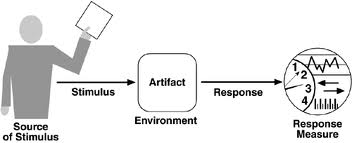
\includegraphics{pictures/qualityAttribute.jpg}
\end{figure}

{\bf What is a quality attribute?:}

{\bf Priority of quality attributes:} It is not possible to meet all quality requirements because some 
decisions will affect the other. This will result in a priority of the quality attributes that we need 
to meet and some others that are not that important. We have picked two main quality attributes: 
modifiability and performance.

\begin{itemize}
	\item {\bf Primary quality attribute: } Modifiability
	\item {\bf Secondary quality attributes: } Performance
\end{itemize}


\subsubsection{Modifiability}

Modifiability is about the cost of change. It brings up two concerns: What can change (the artifact)? 
When is the change made and who makes it (the environment)? 
Once a change has been specified, the new implementation must be designed, 
implemented, tested, and deployed. All of these actions take time and money, both of which can be measured.
Helgelandskraft (the customer) wanted the possibility for further development on the game. The developers
have to keep in mind that the game are developed in a such way that the customer can continue
the development after the delivery. If the game is made in a way that changes are hard to implement, 
the customer would need to use a lot of resources in sense of time and money, and that is the main 
reason for this to be the primary quality attribute.

Changes the customer might want to add to the game is more buildings and more obstacles to take
the game to a more complex state. We have therefore added good models so it would be easy for 
the customer to make further development on this part.

\subsubsection*{M1: Add new elements}
In our game we have specified a small set of elements like powerplants, houses, powerlines, etc.
In order to have the oppertunity to add new buildings we have made a model for each element
with specific attributes. When e developer wants to add more elements, he/she can use the model
we have made and easily add the wanted parameters. 

\begin{tabular}{| l | l |}
	\hline
	{\bf Portion of scenario} & {\bf Values} \\ \hline
	Source of stimulus & Developer\\ \hline
	Stimulus & add new elements to the game\\ \hline
	Environment & design time \\ \hline
	Artifact &  code \\ \hline
	Response & modification is made with no side effects\\ \hline
	Response Measure & 1 hour\\ \hline
\end{tabular}

\subsubsection* {M2: Increase game difficulty}
If the game is made to easy for the user it is possible for the developer to just ajust the
parameters in the models. The difficulty of the game is based on the parameters
in the models. 

\begin{tabular}{| l | l |}
	\hline
	{\bf Portion of scenario} & {\bf Values} \\ \hline
	Source of stimulus & Developer\\ \hline
	Stimulus & modify the difficulty in the game\\ \hline
	Environment & design time \\ \hline
	Artifact & code \\ \hline
	Response & modification is made with no side effects\\ \hline
	Response Measure & 1 hour\\ \hline
\end{tabular}

\subsubsection{Performance}

\subsubsection*{P1: Rendering (Repaint)}
When changes occure to the game models, the screen should identify if the change 
is visible on the screen. If the change can be seen, the screen should repaint 
that part of the display at the beginning of the next game update.

\begin{tabular}{| l | l |}
	\hline
	{\bf Portion of scenario} & {\bf Values} \\ \hline
	Source of stimulus & Game models\\ \hline
	Stimulus & Change to the internal state of game model\\ \hline
	Environment & Game run time \\ \hline
	Artifact &  Game \\ \hline
	Response & Identify visibility of state change\\ \hline
	Response Measure & Less than 16 ms\\ \hline
\end{tabular}

\subsubsection{Other Quality attributes}
\subsubsection*{Usability: } the group do not have the main focus on this quality attribute, 
but since this is a game that is supposed to be played by a varaity of people, it
have to be considered to make the game easy to use. In the game we have added a 
instruction in the main menu so the user can get help to get started.

\subsubsection*{Testability: } since the game are made as a prototype, we have focused on have
test on the main functionality so the customer can run test under further developing.
In order to have test, we need to write testable code.

\subsubsection*{Compitability: } the game has to run on a different kind of platforms. we
have chosen to develop on a cross-platform framwork so it it easier to adapt to 
new platforms.
